\epigraph{\emph{
  ``Coming up with features is difficult, time-consuming, requires expert knowledge. "Applied machine learning" is basically feature engineering.''
}}{ Andrew Ng }

Considering the ``right'' features for clustering is a demanding and error prone process. Currently there is really just one way of describing documents: The vector space model. It breaks down to counting occurences and cooccurences of words and measuring distance by mathematical functions. We could just take all the words of a document, removing stopwords, and put them into a feature vector. This results in dimensionality explosion and extreme noise. Contrary to a document vector $d = \{w_1,w_2..w_n\}$, the feature vector represents a document by concepts $\{c_1,c_2,..c_j\}$. It is a projection of the original document often by fewer dimensions and a lifting of words. This lifting is bestly described as combining several words of a document, often occuring in the same sentence, extracting a shared meaning. We hope to find fewer words that share enough information with the original word, that the following holds:
  
  \begin{equation}
    f : d=\{w_1,w_2,..w_n\} \to \{c_1,c_2,..c_j\}
  \end{equation}

The function $f$ transforms a sequence of words $w_1..w_n$ of a document $d$ to a sequence of concepts $c_1..c_j$. The concepts can be derived in a lot of ways.

  \begin{enumerate}
    \item Pruning words of low and high significance.
    \item Using syntactic parsing to retrieve noun phrases, named entity tags or part of speech tags.
    \item Using ontologies of wordnet to derive a shared meaning of words.
    \item Mapping documents to wikipedia categories.
    \item Using kernel methods, preselecting initial clusters in a semi-supervised way.
  \end{enumerate}

In the end, feature selection is probably the most demanding task. Expert knolwedge needs to be applied and can change over time. A computer handles documents in vector space, by counting. A human however perceives content differently. For any sufficiently adavanced algorithm that works with a knowledge base it is still: Garbage in, garbage out. More fancy algorithms will only lead to more fallacies in selecting the features. Complexity goes down when algorithms are simple and the selection of features is fine tuned.\\

In the following we will briefly explain what \emph{semantics} mean, especially in the \emph{domain} of newspapers. How \emph{feature selection} generally works and how this can be enhanced by \emph{syntactic parsing}. Strategies using \emph{Wordnet} and \emph{Wikipedia} are explained. In the experimental chapter we will then present how all these mechanisms come together.


\section{Semantics}
  
  Semantics is the study of meaning. Given some symbols, characters, words or phrases what is their underlying meaning? The question is inherently hard and lots of literature focuses on how computers can get better at this. Semantics can also be viewed from a statistical point of view. Given a lot of phrases and words, can we infer their underlying structure that generated them? How can statistical patterns reveal what was meant and to what degree?\\
  In computational linguistics we often speak of \emph{word-sense disambiguation (WSD)}. \emph{WSD} is short for identifying sense of a word in a sentence or paragraph. The sentence\\ 

    \emph{``The bail out during the financial crisis of the Lehmann brothers bank, was much too late.''}\\

  makes it obvious that it is about financial institutions ``bank'' during the financial crisis, political intervention by providing money ``bail out'' and a specific financial institution or entity ``Lehmann brothers''. How could we possibliy discern such a sentence so that we can actually reveal all the beforementioned concepts? To successfully find such concepts we have to identify what parts of speech, e.g. nouns, verbs, adjectives etc., each word of a document has:

    \begin{equation}
      pos\-tag(d=[w_1,w_2,..w_n]) = [(w_1, tag_1), (w_2, tag_2),.. (w_n, tag_n)]
    \end{equation}

  For clustering we want to identify these \emph{semantic fields}, a set of words grouped by meaning. We then often analyze \emph{WSD} through \emph{synonymy, polysemy, hyponymy, hypernymy and meronymy}. All of those concepts are important to taxonomies and ontologies. A \emph{taxonomy} is refered to as a simple hierarchical structure of parent-child relationships, that change in granularity per hierarchy level. An \emph{ontology} is much broader and can have complex relations other than parent-child. In that sense both taxonomies and ontologies are structures, showing how to classify words in context to each other. Traversing through these hierarchical structures is typically done by hyponyms and hypernyms. 

    \begin{figure}[h!]
      \centering
        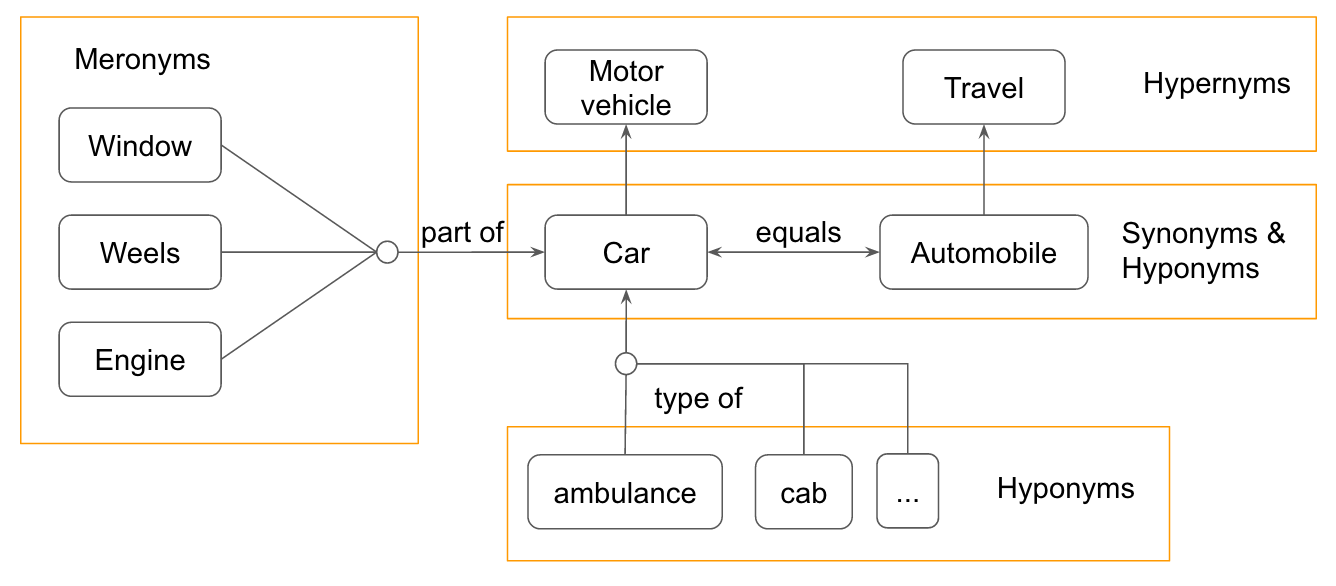
\includegraphics[width=0.7\textwidth]{wsd_analysis.png}
        \caption{"Semantic fields, hierarchies"}
        \label{wsd_analysis}
    \end{figure} 

  \emph{Meronyms} are ``part-of'' relations, \emph{hyponyms} have a ``type-of'' relation to a higher concept, called \emph{hypernyms}.

  \subsection{Domain}
    Newspaper Article, Categories, Metadata

\section{Selection}
  \subsection{Syntactic parsing}
  
\section{Wordnet}

\section{Wikipedia}
  

